\chapter{力学性能试验与组织表征}

\section{力学试验}
力学性能是表征材料性能的重要参数,本次试验\footnote{实验(Experiment)是通过实际操作来探究某一自然或社会规律,主要强调与理论研究的方法对立;而试验(test)采用测试的手段来获取或验证某一结果的行为。此处当为“试验”。}采用常规的拉伸试验来测量式样的力学性能。力学拉伸试验是一种常用的材料力学性能测试方法,用于评估材料的抗拉性能、塑性性能和断裂性能等。其主要特点是通过拉伸试验机对试样进行一定的力量加载和拉伸,测量试样在不同载荷下的应变和应力,以此计算出力学特性参数,如屈服强度、抗拉强度、延伸率等。该测试方法简单、直观,结果可靠,并可以广泛应用于各种材料试样的力学性能评估。本试验根据拉伸试验主要根据测量结果来评估材料的如下四个力学性能指标:
\begin{enumerate}
	\item 屈服强度:表示材料在开始发生可见塑性变形前的最大应力值。
	\item 抗拉强度:表示材料在断裂前所能承受的最大应力值。
	\item 断裂应变:表示材料在断裂发生前所受的最大应变值。
	\item 延伸率:表示材料在断裂前可以发生的塑性变形程度,是反映材料延展性能的指标\footnote{由于试样较小,测量误差大,本设计主要考虑沿拉伸方向的延伸率来分析正应力与正应变,断裂截面较小,界面面积与切应力难以测量,为了保证试验整体的准确性,不对其进行探讨。}。
\end{enumerate}
\subsection{试验设备}

本设计采用拉伸试验机对经固溶时效热处理工艺的试样进行常温微拉伸性能测试。由于试样较小,冲击韧性较差,容易被拉断,为了尽可能准确地观察其力学特性,采用了较慢的$ 0.5mm/min $的拉伸速率来拉伸,每组试样进行两次测定,取其平均值作为最终结果。所用的设备为\text{\color{black}CMT5105}微机控制电子万能试验机(Electromechaniacl Universal Testing Machine),外观如\ref{fig:mymechyest}所示,设备规格如\ref{sec: mymechyest}所示:
\begin{table}[htbp]
	\centering
	\caption{\text{\color{black}CMT5105}微机控制电子万能试验机的规格}
	\label{sec: mymechyest}
	\begin{tabular}{cc}
		\toprule
		参数&值\\
		\midrule
		型号&CMT5105\\
		编号&17020836\\
		电压&三相 380VAC\\
		功率&1.3KW\\
		最大力&100kN\\
		准确度等级&0.5级\\
		制造日期&2022年8月\\
		制造商& $\text{美斯特工业系统}^\text{\textregistered} $(中国)有限公司\\
		\bottomrule
	\end{tabular}
\end{table}

\begin{figure}[h!]
	\centering
	\subfigure[力学试验机]{
		\label{fig:mymechyest}
		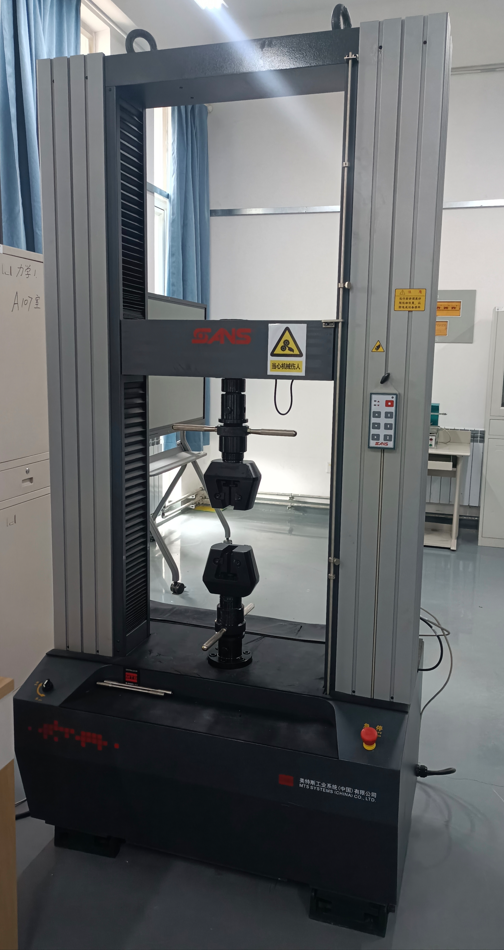
\includegraphics[scale=0.4]{pic/力学试验机}}
	\hspace{0.5in} % 两图片之间的距离
	\subfigure[试样安装]{
		\label{fig:mytest}
		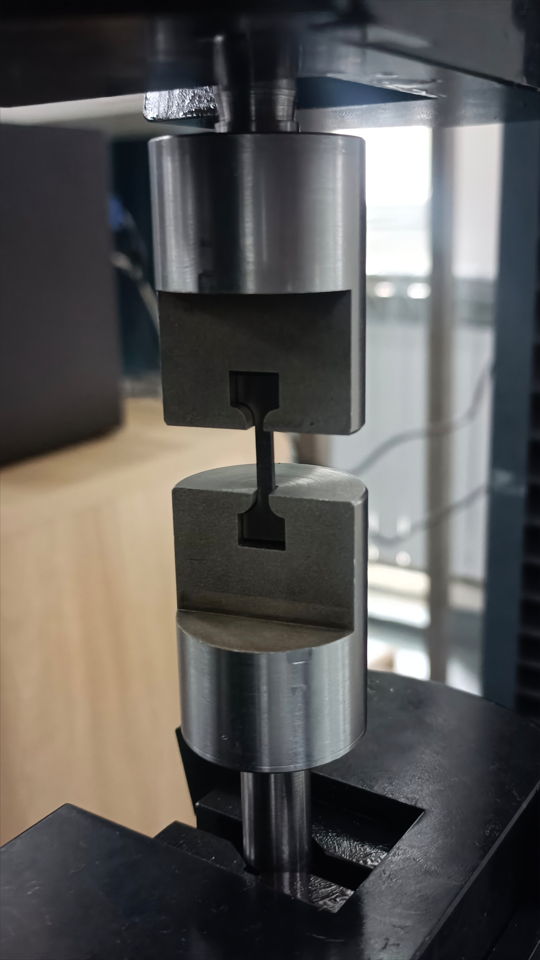
\includegraphics[scale=0.4]{pic/拉伸试验}}
	\caption{拉伸试验}
	\label{fig:拉伸试验}
\end{figure}
\subsection{试验过程}
试验前,先准备好试样,在试样上刻上标记,以确定试样的方向。然后如图\ref{fig:拉伸试验}在拉伸试验机上安装试样,并在拉伸试验机上设置截面尺寸、最大加载力、加载速率等参数。

一次拉伸试验包括两个阶段:弹性阶段和塑性阶段。弹性阶段是指当外力作用在试样上时,试样的形变是可逆的,即当外力消失时,试样会完全恢复其原始尺寸。随着外力的增加,试样进入塑性阶段,此时试样发生不可逆的塑性变形,当外力达到试样的最大强度时,试样会断裂。

试验时,对试样采用一次性拉断的方式来进行测试,并通过传感器,利用计算机来记录其载荷-位移曲线,导出数据进行分析。

最后通过测量式样拉断后的长度,计算得到延伸率。

\subsection{拉伸试验结果分析}
根据对万能力学试验机上测试得到的数据进行整理,得到了抗拉强度\footnote{根据《金属材料室温拉伸试验方法》GBT228-2002,抗拉强度符号已经由$ R_m $代替旧国标中的$ \sigma_b $,故在此使用最新标准$ R_m $来表示抗拉强度。}、延伸率,如\ref{sec:mystrength}所示。又通过去除力学试验数据中从断裂瞬间到试验结束之间的无用数值、整合每组两个试验结果(取平均值),计算得到了试样断裂区域截面($ 1.3mm\times2.5mm=3.25mm^2 $)的应力与应变曲线(拉伸变形量与拉伸区域长度的比值),最后把包括未处理的对照组在内的十组数据的应力应变曲线进行汇总,得到了如\ref{fig:试样应力应变曲线汇总}\footnote{图形中标签未标明的,所有组共同具有工艺参数为:固溶处理时间:10分钟;时效处理时间:60分钟}所示的可视化图形:
\begin{table}[htbp]
	\centering
	\caption{\ti 合金的力学性能试验结果}
	\label{sec:mystrength}
	\begin{tabular}{cccc}
		\toprule
		试验编号& 代号&$ R_m $(Mpa)&延伸率 \\
		\midrule
		0 & 甲 & 1008.69 & 6.83$\%$ \\
		1 & 乙 & 1016.21 & 3.73$\%$ \\
		2 & 丙 & 1077.33 & 4.24$\%$ \\
		3 & 丁 & 1052.72 & 3.49$\%$ \\
		4 & 戊 & 1099.33 & 2.60$\%$ \\
		5 & 己 & 1113.90 & 2.57$\%$ \\
		6 & 庚 & 1077.28 & 2.88$\%$ \\
		7 & 辛 & 790.10 & 1.94$\%$ \\
		8 & 壬 & 799.54 & 2.05$\%$ \\
		9 & 癸 & 873.38 & 2.19$\%$ \\
		\bottomrule
	\end{tabular}
\end{table}
\begin{figure}[h!]
	\centering
	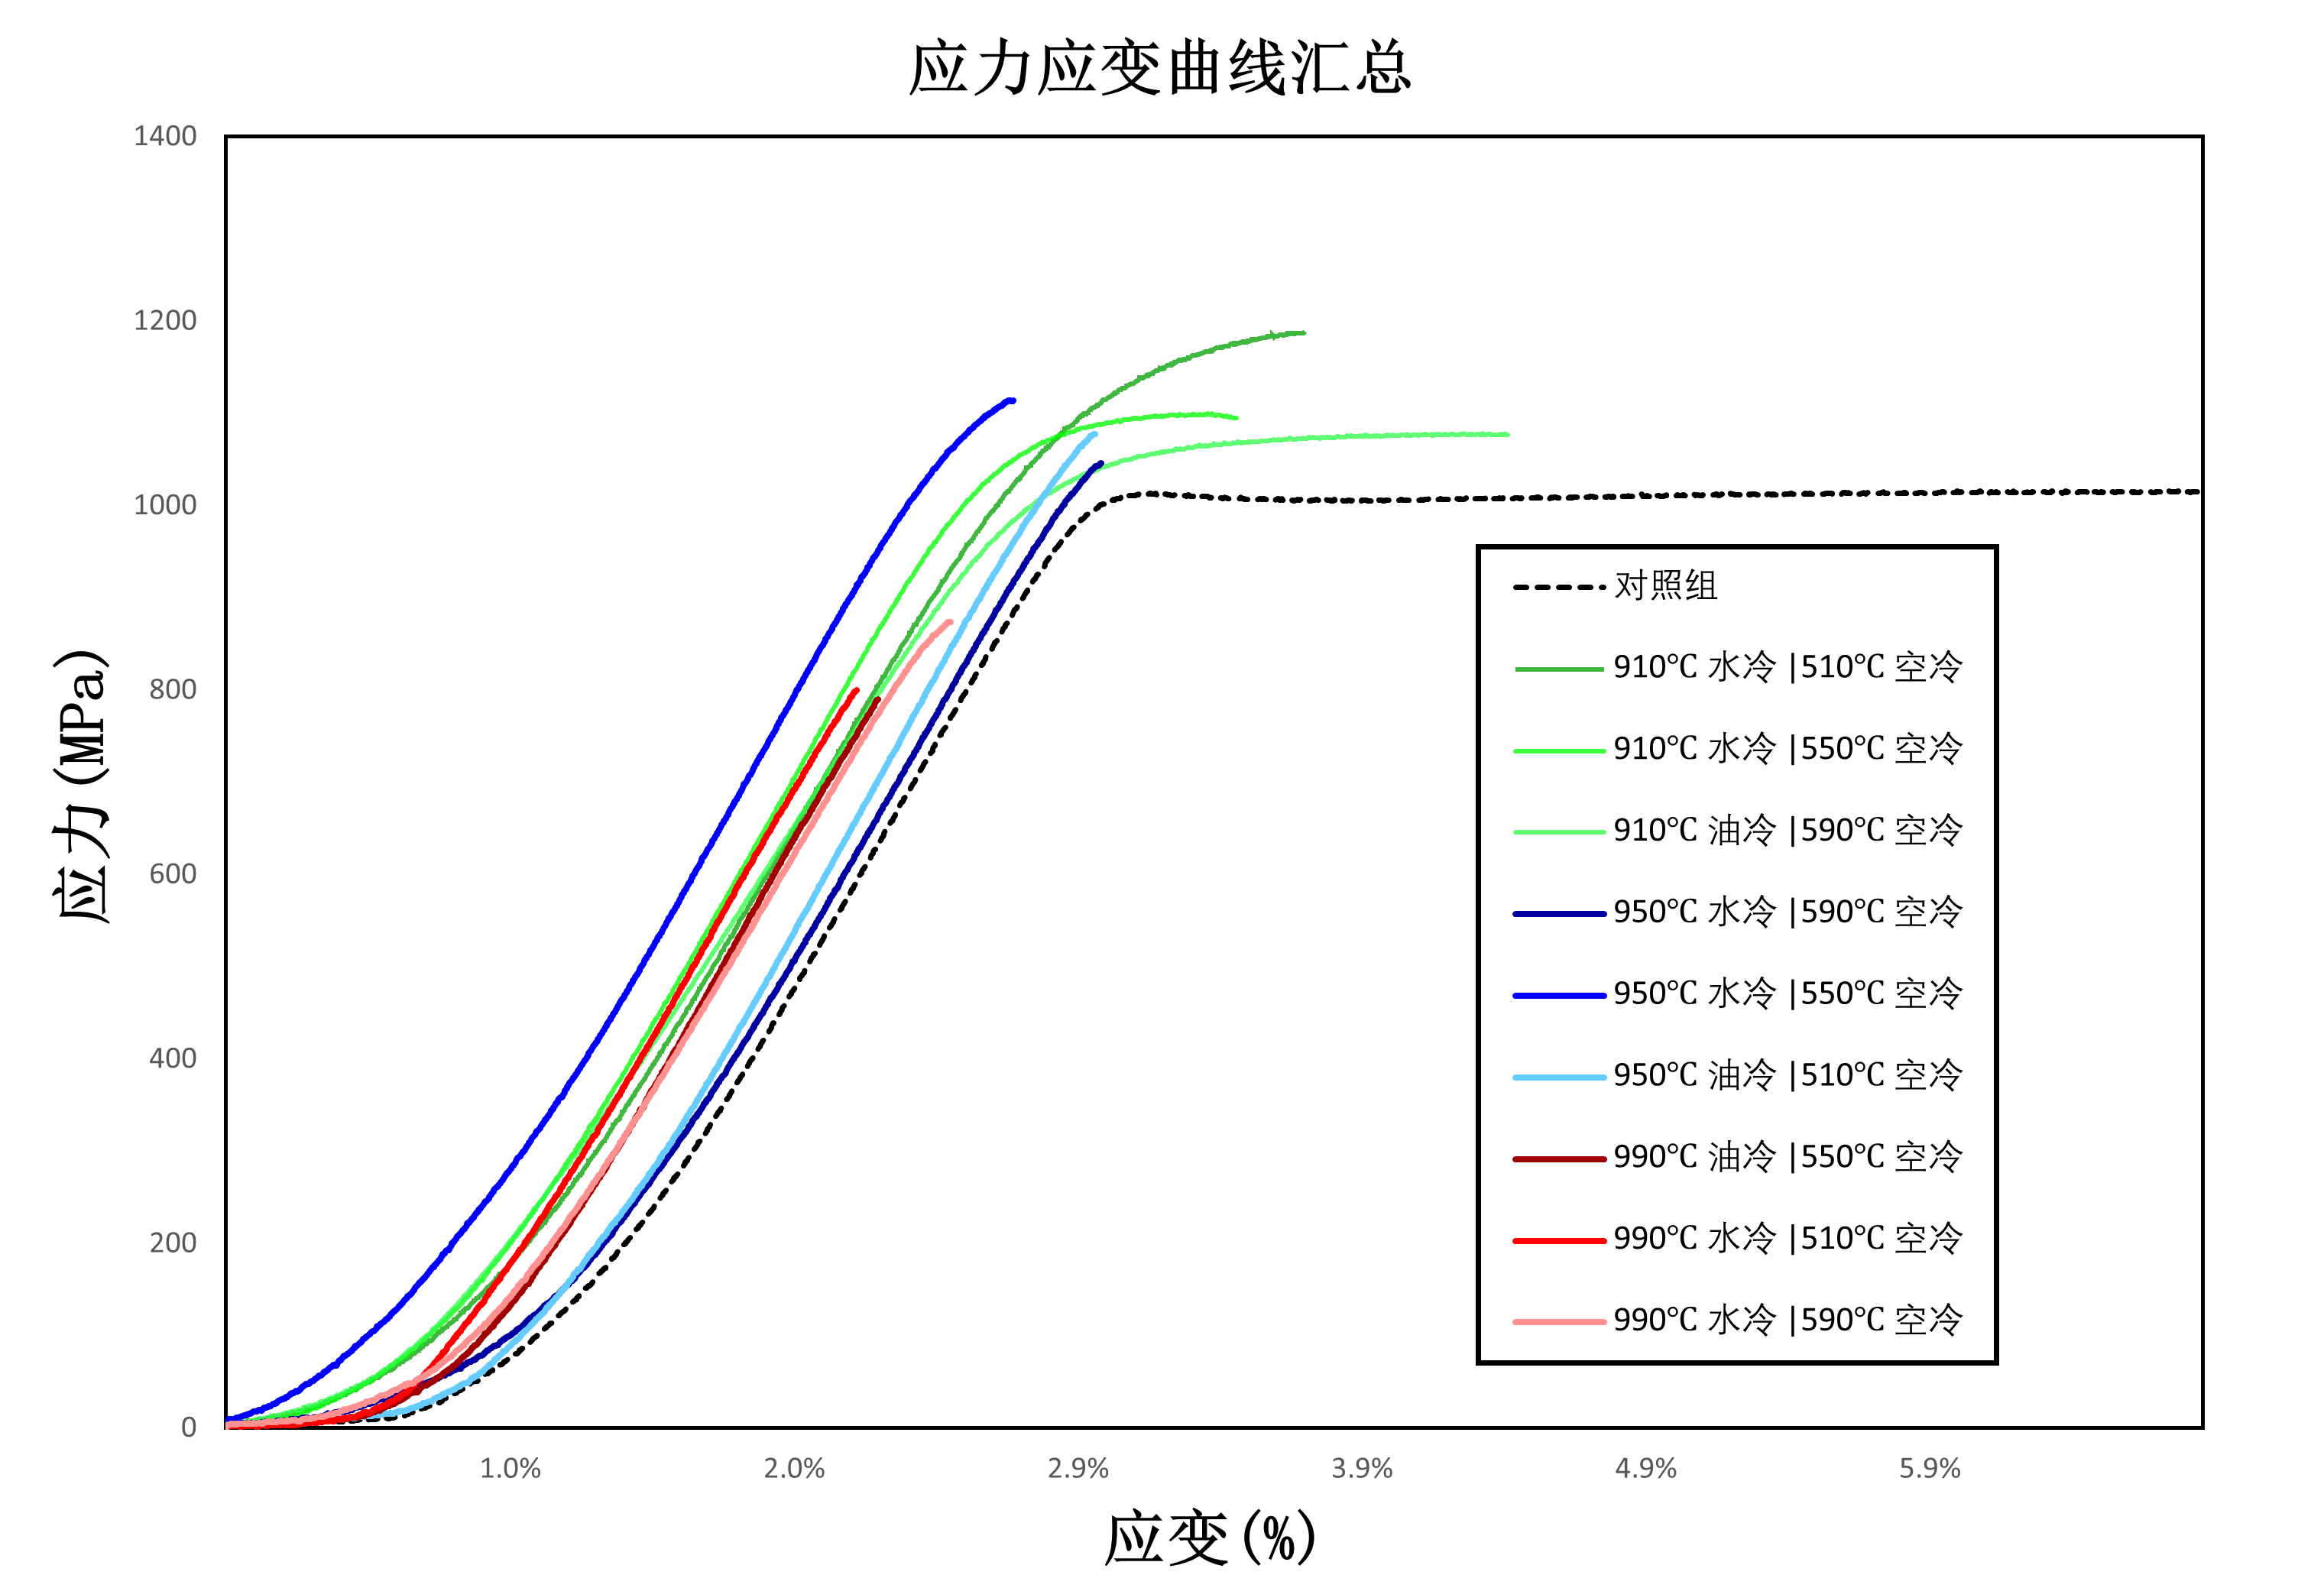
\includegraphics[width=0.99\linewidth]{pic/试样应力应变曲线汇总.png}
	\caption{试样应力应变曲线汇总}
	\label{fig:试样应力应变曲线汇总}
\end{figure}

从图中经过分析可以看出:固溶-时效处理后试样对材料各方面的影响还是比较明显的。力学性能对比分析如下
\begin{enumerate}
	\item \textbf{整体塑性降低:}与对照组相比,910℃固溶组塑性大幅度降低,在经过短暂的屈服阶段后即被拉断;950℃、990℃固溶组的塑性更低,几乎呈现出来脆性材料的特点,断裂都属于脆性断裂。
	\item \textbf{抗拉强度有所提升:}910℃、950℃固溶组的抗拉强度与对照组相比都有所提升,其中以910℃固溶+510℃空冷组的强度为最高。
	\item \textbf{固溶温度较高时,强度有所降低}990℃固溶组的强度、塑性降低最为明显,990℃固溶+550℃空冷组的抗拉强度已经降低到了$ 790Mpa $左右,990℃固溶+510℃空冷组的最大应变达到了$ 2.18\% $,几乎是对照组$ 6.83\% $的三分之一。
\end{enumerate}


\section{显微组织表征}
现阶段常用于观察组织和分析相结构的检测方法主要包括:光学显微镜 (OM)、扫描式电子显微镜 (SEM)、X射线衍射分析 (XRD)以及透射式电子显微镜 (TEM)等。

将固溶与时效后的试件进行线切割截取显微组织分析试样,截取后的试样进行 150\#、400\#、1000\#、1500\#、2000\#、2500\#金相砂纸磨制,对磨制后的试样采用 0.05umSiO2抛光液在抛光机上进行抛光,去除试样表面的划痕或杂质颗粒,经抛光后的试样采用$ HF:HNO3:H2O=2:4:94 $的Kroll试剂进行腐蚀。腐蚀后的试样分别采用光 学显微镜(OM)、扫描电子显微镜(SEM)对其微观形貌进行观察。

\section{式样的显微组织表征与结果分析}
三种不同固溶温度得到的试样组织如下:
\begin{figure}[h!]
	\centering
	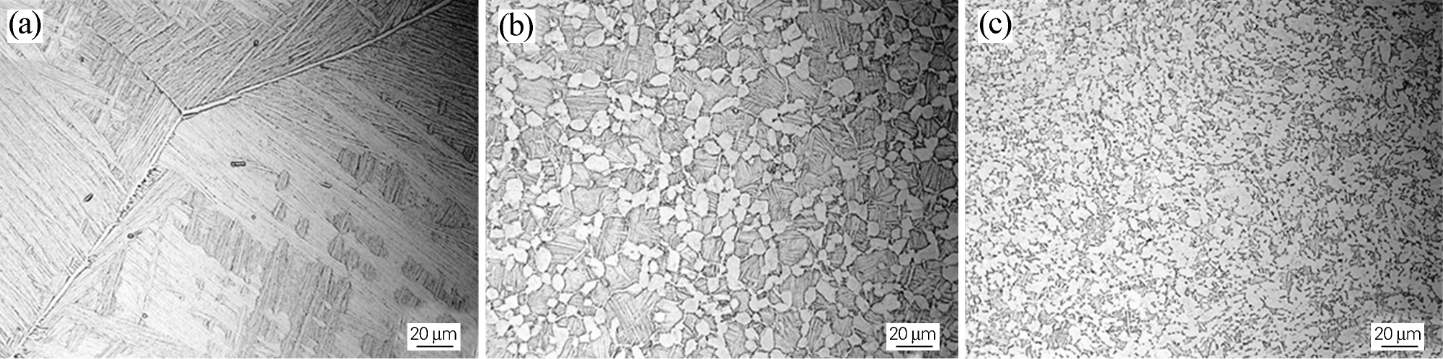
\includegraphics[width=0.7\linewidth]{pic/demo-mico}
	\caption{不同热处理工艺下 TC4 钛合金的显微组织}
	\label{fig:demo-mico}
\end{figure}